\section{Experiments}
Our goal was to reproduce the main experiment in (mention paper here) and also, perform our own experiment and compare our results. We followed the model proposed in the paper, but instead of using the tensorflow framework, we used pytorch. (Time for training and testing are not very relevant, since the network is shallow, only two layers, and it takes less than 30 seconds to perform such tasks.) 

\subsection{Datasets}

Following the experiments of (mention paper here again), we used 3 of their 4 datasets from citation networks: Cora, Citesser and Pubmed. The three datasets are set up where the nodes are papers (documents) and the edges are citation links. In Table ~\ref{tab:datasets} we have the datasets statistics. Training can only be done in nodes that have labels, in our case there are 20 nodes per class for each dataset, the total number per dataset is shown in the trainable nodes column.

\begin {table}[ht]
\caption {Datasets} \label{tab:datasets} 
  \begin{center}
    \begin{tabular}{|c|c|c|c|c|}
    \hline
    Dataset  & Nodes  & Classes & Features & Trainable nodes\\
    \hline 
    Cora     & 2,708  & 7       & 1,433    & 140 \\ 
    Citeseer & 3,327  & 6       & 3,703    & 120  \\  
    Pubmed   & 19,717 & 3       & 500      & 60   \\
    \hline
    \end{tabular}
  \end{center}
\end{table}

\subsection{The Model}
The model utilized by the authors' is a 2-layer convolution network, and the model can be represented by Equation -- .
\begin{align*}
    f(x,A) &= softmax(\hat{A}ReLU(\hat{A}XW_{0})W_{1})
\end{align*}

Figure \ref{fig:model} illustrates the set up.

The first layer takes as input a matrix $x_{0}$ that contains the features of the data. This matrix is used to calculate the dot product with the \textit{normalized adjacency matrix} $\hat{A}$ and the weight matrix $w_{0}$. After the dot product is done the result is passed through the \textit{RelU}activation function, and the result matrix is used as input $x_{1}$ for layer 2.

In layer 2, $x_{1}$ that comes from layer one is used to calculate the dot product with the same \textit{normalized adjacency matrix} and a matrix of weights $w_{1}$.

The matrix generated by the second matrix is passed through a \textit{softmax} so the data can be classified into the classes.

\begin{figure}[h!]
  \centering
  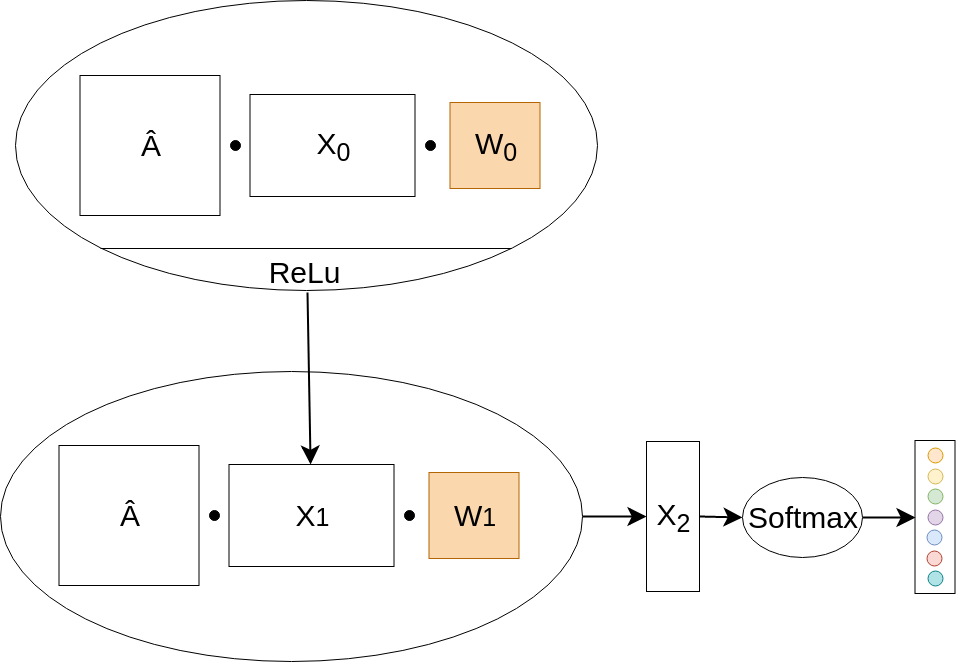
\includegraphics[width=0.8\linewidth]{media/model.png}
  \caption{Graph Convolution Network}
  \label{fig:model}
\end{figure}

\subsection{Experiment 1}

We reproduced the authors' experiment with  the hyperparameters presented in Table \ref{tab:hyperparameters1}.

\begin {table}[ht]
\caption {Hyperparameters Experiment 1} \label{tab:hyperparameters1} 
  \begin{center}
    \begin{tabular}{|c|c|}
    \hline
    Learning rate     & 0.001 \\ 
    Epochs            & 200  \\ 
    Optimization      & ADAM \\
    Drop out          & 0.5   \\
    Weight Decay      & 0.0005 \\
    regularization    & L2    \\
    \hline
    \end{tabular}
  \end{center}
\end{table}

\subsection{Experiment 2}
In experiment 2, we trained the Cora dataset and fine tuned our own hyperparameters as presented in Table \ref{tab:hyperparameters2}.

\begin {table}[ht]
\caption {Hyperparameters Experiment 2} \label{tab:hyperparameters2} 
  \begin{center}
    \begin{tabular}{|c|c|}
    \hline
    Learning rate     & 0.001 \\ 
    Epochs            & 200  \\ 
    Optimization      & ADAM \\
    Drop out          & 0.5   \\
    Weight Decay      & 0.0005 \\
    regularization    & L2    \\
    \hline
    \end{tabular}
  \end{center}
\end{table}